\section{Forward Time Projection Chamber (FTPC)}

	Οι Time Projection Chambers (TPCs) είναι μία υποκατηγορία των θαλάμων ολίσθησης. 
	%Αποτελούνται από μία κοιλότητα η οποία περιέχει ένα αέριο και κάποια λεπτά σύρματα Εφαρμόζοντας ηλεκτρικό (μέσω διαφοράς δυναμικού στα σύρμαυα) και μαγνητικό πεδίο (από εξωτερικές πηγές) στον χώρο του αερίου μπορούμε να κατευθύνουμε τα φορτισμένα σωματίδια που υπάρχουν. 
	Αποτελούνται από μία κοιλότητα, στην περίπτωσή μας κυλινδρική, η οποία περιέχει ένα αεριο. Εντός αυτής της κοιλότητας επιβάλλουμε ηλεκτρικό πεδίο προς τις βάσεις του κυλίνδρου ( μέσω δύο μεγάλων ηλεκτροδίων ) και εξωτερικό μαγνητικό πεδίο παράλληλο με το ηλεκτρικό.
	Τότε, τα σωματίδια που περνάνε εντός της κοιλότητας και έχουν ιονιστική ικανότητα, υπό κατάλλες συνθήκες πίεσης και τιμές των πεδίων, ιονίζουν τα άτομα/μόρια του αερίου, δημιουργείται το φαινόμενο Townsted και ανιχνεύονται ως ένα σήμα μετά τους Multiwire  Proportion Chambers (MWPC)  στους Readout Chambers που είναι τοποθετημένοι σε μπλοκ στις δύο βάσεις. Οι MWPC είναι περιοχές που αποτελούνται από σύρματα-ανόδους πριν την τελική κάθοδο προκειμένου να ενισχυθεί το σήμα. Η λειτουργία τους θα περιγραφεί αναλυτικότερα στην συνέχεια όπου θα μελετήσουμε τους συμβατικούς TPC.
	Από την θέση που ανιχνεύονται τα σήματα μπορούμε να προσδιορίσουμε την προβολή της τροχιάς στις βάσεις και από την χρονική διαφορά που υπάρχει μεταξύ των ανιχνεύσεων μπορούμε να προσδιορίσουμε και την τρίτη συνιστώσα της τροχιάς. Ταυτόχρονα μπορούμε να ταυτοποιήσουμε τα σωματίδια μέσω της ενέργειας που εναποθέτουν στο αεριο μέσω ιονισμού ( Καμπύλη Bethe-Bloch).
	
	
	 Συγκεκριμένα οι FTPC του STAR έχουν κάποιες ιδιαιτερότητες οι οποίες προέκυψαν προκειμένου να επεκταθεί η κάλυψη σε μεγαλύτερες τιμές pseudorapidity $2.5<|\eta|<4.0$ καθώς υπήρχε η ανάγκη για κάλυψή τους αφού παράγονταν υψηλές πυκνότητες σωματιδίων με μεγάλη η. Η pseudorapidity πρόκειται για μία χωρική συντεταγμένη η οποία περιγράφει την γωνία ενός σωματιδίου που παράγεται από τις κρούσεις ως προς την αρχική δέσμη και ορίζεται ως 
	 	\begin{equation}\label{eq3.1}
	 		\eta = -ln\left(tan(\theta/2)\right) = arctanh(\frac{p_L}{|\bm{p}|} )
	 	\end{equation}
	 	
	 	όπου θ η γωνία δέσμης-ορμής σωματιδίου, $|\bm{p}|$ το μέτρο της ορμής του και $p_L$ η συνιστώσα της ορμής που είναι παράλληλη στην δέσμη. Άρα οι FTPC στόχευαν  να βελτιώσουν τον χαρακτηρισμό των γεγονότων στο STAR ανιχνεύοντας σωματίδια με μιρκή γωνία θ προς την δέσμη και επιτρέποντας την μελέτη μη συμμετρικών συκγρούσεων όπως Au-p. 
	 	
	 	\subsection{Η λειτουργία των FTPC}

	Οι FTCP του STAR διαφέρουν σε μερικά σημεία από έναν απλό TPC. Η ιδέα γι' αυτούς καθορίστηκε από δύο παράγοντες. Πρώτον, την ανάγκη για κάλυψη μεγάλων η και δεύτερον τον περιορισμένο χώρο μεταξύ δέσμης και του κανονικού TPC που υπάρχει μετά τον FTPC. 
	Όπως φαίνεται στην Εικόνα (\ref{fig3.2}) πρόκειται για ένα κυλινδρικό θάλαμο εσωτερικής ακτίνας $R_{FTCP,in}=7.73cm$, εξωτερικής ακτίνες $R_{FTCP,out}=30.05cm$, μήκους $L_{FTCP}=120cm$ με ακτινικό πεδίο ολίσθησης που προκαλείται από την διαφορά δυναμικού $10-15kV$ μεταξύ του εσωτερικού και εξωτερικού ηλεκτροδίου. Έτσι, οι  Readout Chambers είναι τοποθετημένοι σε 5 κυλινδρικά δαχτυλίδια στην εξωτερική επιφάνεια τoυ FTCP. Καθένα από τα δαχτυλίδια έχει 6 Readout Chambers.
	
	\begin{figure}[h!]
		\centering
		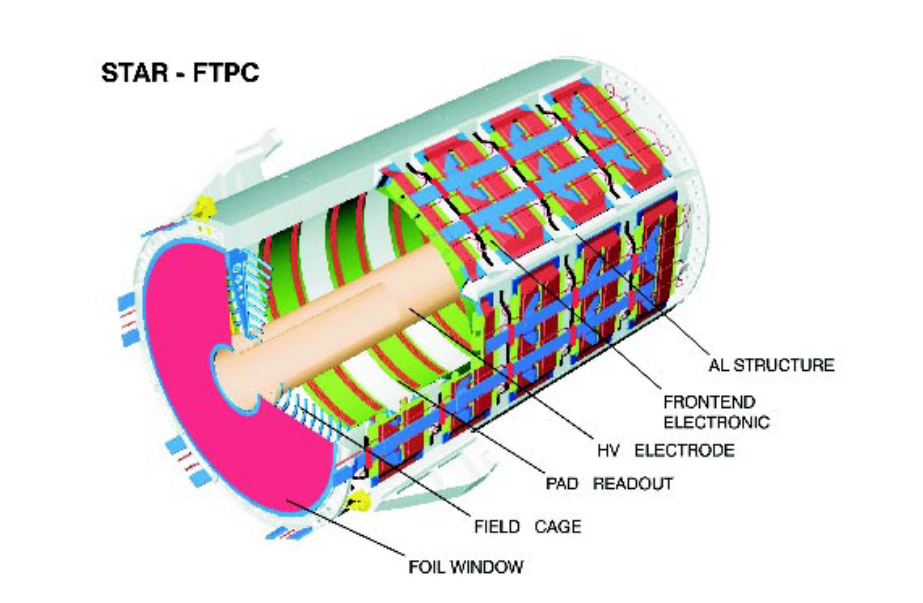
\includegraphics[scale=0.5]{STAR_Detectors/STAR_FTCP.png}
		\caption{Η δομή του FTCP}
		\label{fig3.2}
	\end{figure}		 	
	 	
	 	
	 Μία από τις ιδιαιτερότητες του FTPC είναι ότι η ολίσθηση των ηλεκτρονίων γίνεται ακτινικά, δηλαδή κάθετα στο μαγνητικό πεδίο, προκειμένου να να βελτιωθεί η διακριση μεταξύ δύο τροχιών κοντά στην δέσμη όπου η πυκνότητα των σωματιδίων είναι μεγαλύτερη. Η προβολή της τροχιάς στην βάση του θα μείωνε την διακριτική του ικανότητα καθώς ο FTPC βρίσκεται πολύ κοντά στην δέσμη και τα σωματίδια δεν θα προλάβαιναν να διαχωριστούν επαρκώς. Την εποχή που κατασκευάστηκε ήταν ο μοναδικός TCP που μπορούσε να διακρίνει δύο τροχιές με ακρίβεια 1-2mm. Ακόμη, έχουν χρησιμοποιηθεί καμπύλοι Readout Chambers (Εικόνα (\ref{fig3.4}) για να διατηρηθεί το ακτινικό ηλεκτρικό πεδίο όσο πιο αναλοίωτο γίνεται. 
	 
	 
	 Το μείγμα αερίων που χρησιμοποιείται είναι Ar/$CO_2$ (50\%-50\%). Αυτό έχει τα πλεονεκτήματα ότι δεν αλλοιώνεται με τον χρόνο, είναι χημικά αδρανές, δεν είναι εύκλεκτο και έχει μικρό συντελεστή διάχυσης για τα ηλεκτρόνια. Το τελευταίο βελτιώνει την χωρική διακριτική ικανότητα, δεδομένου ότι αυτή δίνεται από την σχέση 
	 	\begin{equation}\label{eq3.2}
	 		\sigma_x = \frac{\sigma_D\sqrt{L}}{\sqrt{n}}
	 	\end{equation}
	 όπου $\sigma_D$ ο συντελεστή διάχυσης για τα ηλεκτρόνια, $L$ το μήκος που ταξιδεύουν εντός του αερίου.
	 
	 \begin{figure}[h!]
	 	\centering 
	 	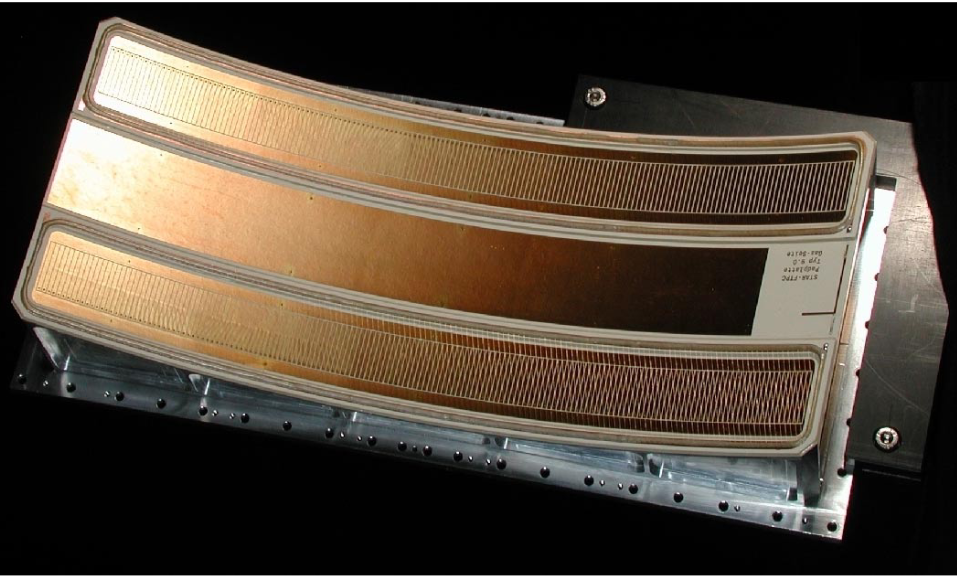
\includegraphics[scale=0.5]{STAR_Detectors/FTPC_readout_chamber}
	 	\caption{Readout Chamber του FTPC. Η ακτίνα καμπυλότητάς του είναι 305mm και έχει δύο συστοιχίες από 160 pad η κάθε μία. }
	 	\label{fig3.3}
	 \end{figure}
	 
	 Προκειμένου να υπάρχει παραγωγή ενός χρήσιμου σήματος από τις καθόδους,  ακριβώς πίσω τους υπάρχουν ηλεκτρονικά, που αποτελούνται συνολικά από 19.200 κανάλια, και τα οποίο λέγονται Front End Electronics (FEΕ). Αυτά ενισχύουν, διαμορφώνουν και ψηφιοποιούν το σήμα. Κάθε pad είναι συνδεδεμένο με έναν προενισχυτή ο οποίος μετά από κάποια στάδια στέλει το σήμα στο Data Aquisition System (DAQ).
	 
	 Κατά την λειτουργία, είναι εμφανές πως οι συνθήκες που επικρατούν δεν είναι συνεχώς ιδανικές και όπως είχαν αρχικά σχεδιαστεί. Γι' αυτό υπάρχει ένα σύστημα Nd:YAG Laser που βοηθά στην βαθμονόμηση και εξετάζει την λειτουργικότητα των FTPC ανεξάρτητα του RHIC. Συγκεκριμένα, προκαλεί ευθύγραμμους ιονισμούς από γνωστές θέσεις προκειμένου να εντοπιστούν τυχών χωρικές διαταραχές που οφείλονται στα μηχανικά χαρακτηριστικά του FTPC ή σε ατέλειες του πεδίου. Βοηθά επίσης στην βαθμονόμηση των ταχυτήτων ολίσθησης του αερίου.
	 	
	 Αφού πλέον μπορούμε να ανιχνεύσουμε τις τροχιές των σωματιδίων μέσω των σημάτων στις ανόδους και να βαθμονομήσουμε το σύστημά μας με την βοήθεια των Laser, θα πρέπει να μπορούμε να επανακατασκευάσουμε τις τροχιές.
	  Το πρώτο στάδιο είναι να εντοπίσουμε τα σημεία των ανόδων που έδωσαν σήμα στα ηλεκτρονικά. Αυτό γίνεται μέσω ενός προγράμματος που διαβάζοντας τα δεδομένα που δίνονται από τα pads, τον χρόνο ολίσθησης και τις απαραίτητες διορθώσεις λόγω της ύπαρξης μαγνητικού πεδίου το οποίο αλλοιώνει την χωρική διακριτική ικανότητα, αντιστοιχεί τις περιοχές μη μηδενικού φορτίου σε συντεταγμένες θέσης. 
	  Το δευτερο βήμα είναι να ομαδοποιήσουμε αυτές τις θέσεις μη μηδενικού φορτίου. Κατασκευάζοντας τις τροχιές, βρίσκει το σημείο τομής τους, το οποίο θεωρούμε ότι είναι το σημείο από το οποίο προήλθαν τα σωματίδια και έπειτα συνδυάζοντας αυτό το σημείο με το μαγνητικό πεδίο υπολογίζονται οι ορμές των σωματιδίων. Μία τέτοια ανακατασκευή φαίνεται στην Εικόνα (\ref{fig3.4}), όπου από 14.745 χωρικά σημεία έχουν ανακασκευασθεί περίπου 1000 τροχιές σωματιδίων σε λιγότερο από 2 δευτερόλεπτα.
	  
	  \begin{figure}[h!]
	  		\centering
	  		\includegraphics[scale=0.5]{STAR_Detectors/FTPC_Reconstruction}	
	  		\caption{Ανακατασκευασμένες τροχιές από τον FTCP προερχόμενες από γεγονότα Au-Au $\sqrt{S}=200GeV$}  
	  		\label{fig3.4}
	  \end{figure}
	  
	  %Συνολικά, η χωρική διακριτική ικανότητα των FTCP είναι 100$\mu m$, η διακριτική ικανότητα στην ορμή βρίσκεται από προσομοίωση 12-15\% 